In this section the results obtained by the face recognition algorithm is  presented. The effects of performing face detection have been ignored in these results.

Table~\ref{tb:fr_results} show the results of applying the face recognition algorithm to the test data set.

\begin{center}
  \captionof{table}{Results of performing face recognition on the test data set.}
  \label{tb:fr_results}
    \begin{tabular}{ | l | l | l | p{5cm} |}
    \hline
    Number of images & False positives & False negatives & Recognition Rate \\ \hline
    78 & 0 & 10 & 86\% \\ \hline
    \end{tabular}
\end{center}

Since the LPQ method used for face recognition is supposedly blur invariant the effects of applying different types of blur to the input images where examined to verify this claim. Figure~\ref{fig:fr_result_plots_gauss} shows how the recognition rate is effected by applying Gaussian blur to the input images while Figure~\ref{fig:fr_result_plots_motion} shows the effect caused by a linear motion blur filter.

\begin{figure}[H]
\centering
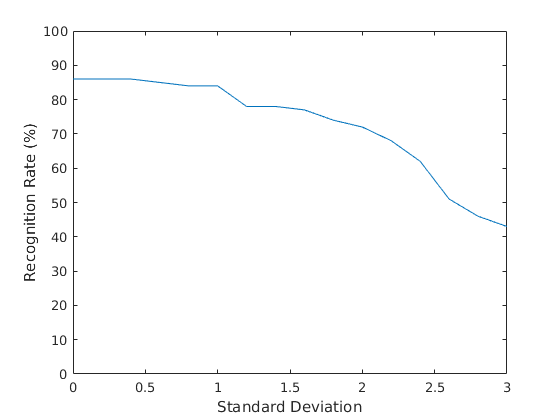
\includegraphics[width=0.8\textwidth]{img/blur_test/gauss_plot.png}
\caption{Shows how applying Gaussian blur effects the recognition rate.}
\label{fig:fr_result_plots_gauss}
\end{figure}

\begin{figure}[H]
\centering
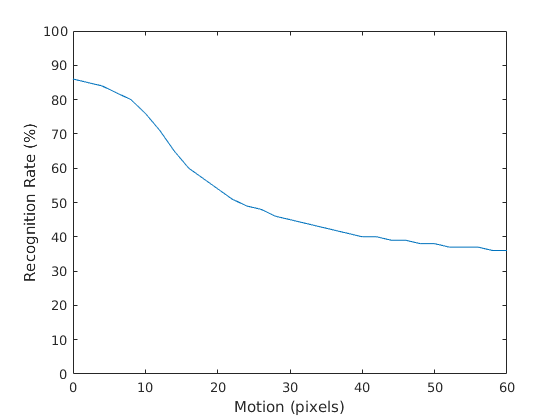
\includegraphics[width=0.8\textwidth]{img/blur_test/motion_plot.png}
\caption{Shows how applying linear motion blur effects the recognition rate.}
\label{fig:fr_result_plots_motion}
\end{figure}

Figure~\ref{fig:fr_result_images} shows what happens to an image after applying Gaussian blur or linear motion blur.

\begin{figure}[H]
\centering
\begin{subfigure}{.30\textwidth}
  \centering
  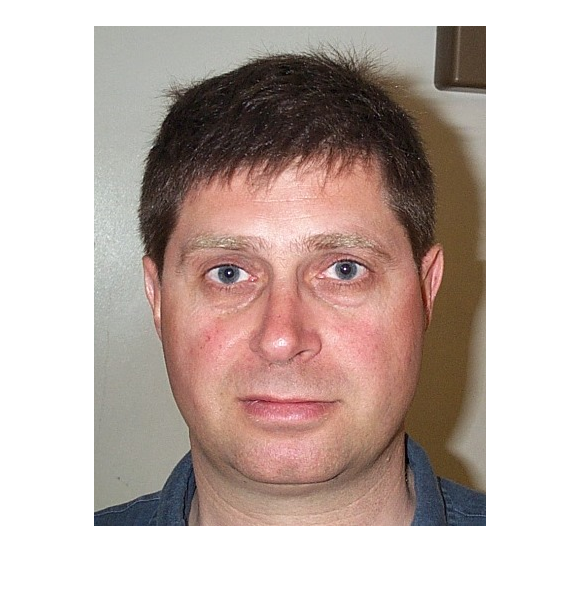
\includegraphics[width=0.8\textwidth]{img/blur_test/orig_img.png}
  \caption{}
\end{subfigure}%
\begin{subfigure}{.30\textwidth}
  \centering
  
\includegraphics[width=0.8\textwidth]{img/blur_test/gauss_img.png}
  \caption{}
\end{subfigure}%
\begin{subfigure}{.30\textwidth}
  \centering
  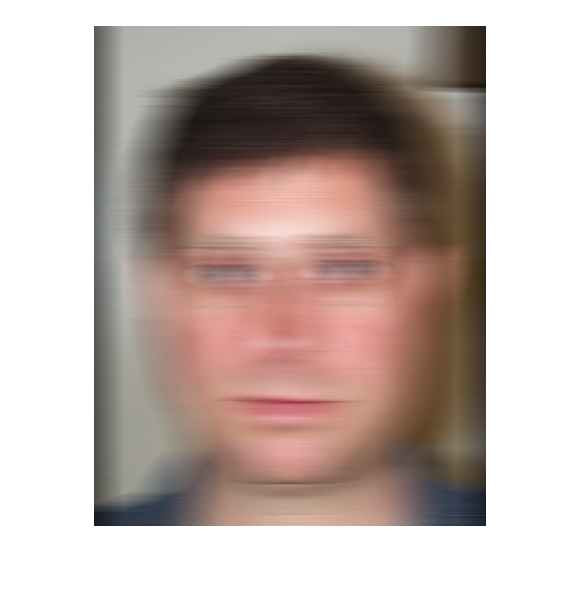
\includegraphics[width=0.8\textwidth]{img/blur_test/motion_img.png}
  \caption{}
\end{subfigure}%
\caption{A comparison of different types of blur applied to the same image. (a) shows the original image. (b) shows the effect of applying Gaussian blur to (a) using a standard deviation of 3.0. (c) shows the result of a 60 pixels wide linear motion blur filter applied to (a).}
\label{fig:fr_result_images}
\end{figure}
